\chapter{Réalisation et Implémentation}
\label{chap:realisation}

\section*{Introduction}
\addcontentsline{toc}{section}{Introduction}
Après avoir défini l'architecture théorique du système, ce dernier chapitre est consacré à la réalisation du projet. Nous y détaillerons l'environnement de développement, les choix d'implémentation spécifiques côté Backend et Frontend, ainsi que les stratégies de sécurité appliquées. Enfin, nous présenterons le résultat final à travers une cartographie des interfaces graphiques de l'application.

% ---------------------------------------------------------
\section{Environnement de Développement et DevOps}
Pour garantir la robustesse et la maintenabilité du code, l'environnement de développement a été standardisé autour d'outils modernes :

\begin{itemize}
    \item \textbf{Gestionnaires de paquets :} Utilisation de \textbf{npm} pour le Frontend (Node.js) et de \textbf{uv} (un gestionnaire ultra-rapide écrit en Rust) pour la résolution déterministe des dépendances Python du Backend.
    \item \textbf{Qualité du code (Linting) :} L'analyse statique du code Frontend est assurée par \textbf{Oxlint} et le compilateur \textbf{TypeScript} (\texttt{tsc}), garantissant l'absence d'erreurs de typage avant la compilation.
    \item \textbf{Conteneurisation (Docker) :} Le Backend et la base de données PostgreSQL sont conteneurisés via \texttt{docker-compose}. L'image de l'API est construite via un \textit{Multi-stage build} afin de minimiser le poids final et de réduire la surface d'attaque.
    \item \textbf{Intégration Continue (CI/CD) :} Un pipeline automatisé sur \textbf{GitHub Actions} exécute les tests unitaires à chaque modification du code et déploie automatiquement l'image sur Docker Hub lors d'une fusion sur la branche principale.
\end{itemize}

% ---------------------------------------------------------
\section{Implémentation du Backend (FastAPI)}

\subsection{Ingestion des Données et ORM Asynchrone}
La couche d'accès aux données de l'API a été développée de manière 100\% asynchrone (non-bloquante) grâce à \textbf{SQLAlchemy 2.0} et au driver \texttt{asyncpg}. 
Le processus d'ingestion en masse (\textit{Bulk Entry}) valide chaque ligne de KPI (type de donnée, existence du projet), attache automatiquement l'auteur de la modification (Administrateur ou Clé d'API), et insère les données de manière atomique (une seule transaction SQL) pour garantir l'intégrité de la base.

\subsection{Sécurité et Hachage Cryptographique}
La protection des données et des accès repose sur le module natif Python \texttt{hashlib} :
\begin{itemize}
    \item \textbf{Mots de passe Utilisateurs :} Hachés selon le standard industriel \textbf{PBKDF2-HMAC-SHA256} avec l'ajout d'un sel cryptographique aléatoire et 100 000 itérations, rendant les attaques par force brute inefficaces.
    \item \textbf{Clés d'API (Principe du \textit{Zero-Knowledge}) :} Lors de la génération d'une clé d'API pour la macro Excel/Script Python, celle-ci n'est affichée qu'une seule fois. Seul un condensat \textbf{SHA-256} est stocké en base de données.
\end{itemize}

% ---------------------------------------------------------
\section{Implémentation du Frontend (React)}

\subsection{Gestion d'état et Cache Serveur}
Plutôt que d'utiliser des états locaux complexes, l'application exploite \textbf{TanStack Query} pour gérer le cache serveur. Les données du Dashboard sont mises en cache de manière intelligente. Cela permet de minimiser les appels à l'API et d'offrir une interface extrêmement réactive lors du changement de filtres temporels.

\subsection{Rafraîchissement Silencieux du Token (Intercepteur Axios)}
Pour offrir une expérience utilisateur fluide (sans déconnexions soudaines), un intercepteur réseau a été développé avec \textbf{Axios} :
Lorsqu'une requête API échoue à cause d'un \textit{Access Token} expiré (Erreur 401), l'intercepteur suspend la requête, utilise le \textit{Refresh Token} en arrière-plan pour obtenir de nouveaux identifiants, met à jour le cache local, puis rejoue la requête initiale de manière totalement transparente pour l'utilisateur.

\subsection{Interface Utilisateur (UI/UX)}
L'interface a été conçue sur mesure à l'aide de \textbf{Tailwind CSS v4}, permettant un \textit{Responsive Design} parfait sans surcharger l'application avec des bibliothèques de composants lourdes. Les graphiques dynamiques sont propulsés par \textbf{Chart.js}, offrant des visualisations claires des tendances hebdomadaires.

% ---------------------------------------------------------
\section{Présentation des Interfaces de l'Application}
Cette section illustre le résultat final du projet à travers les écrans clés de la plateforme HCM-S CIM3.

\subsection{Espace Public et Consultation}

\begin{figure}[H]
    \centering
    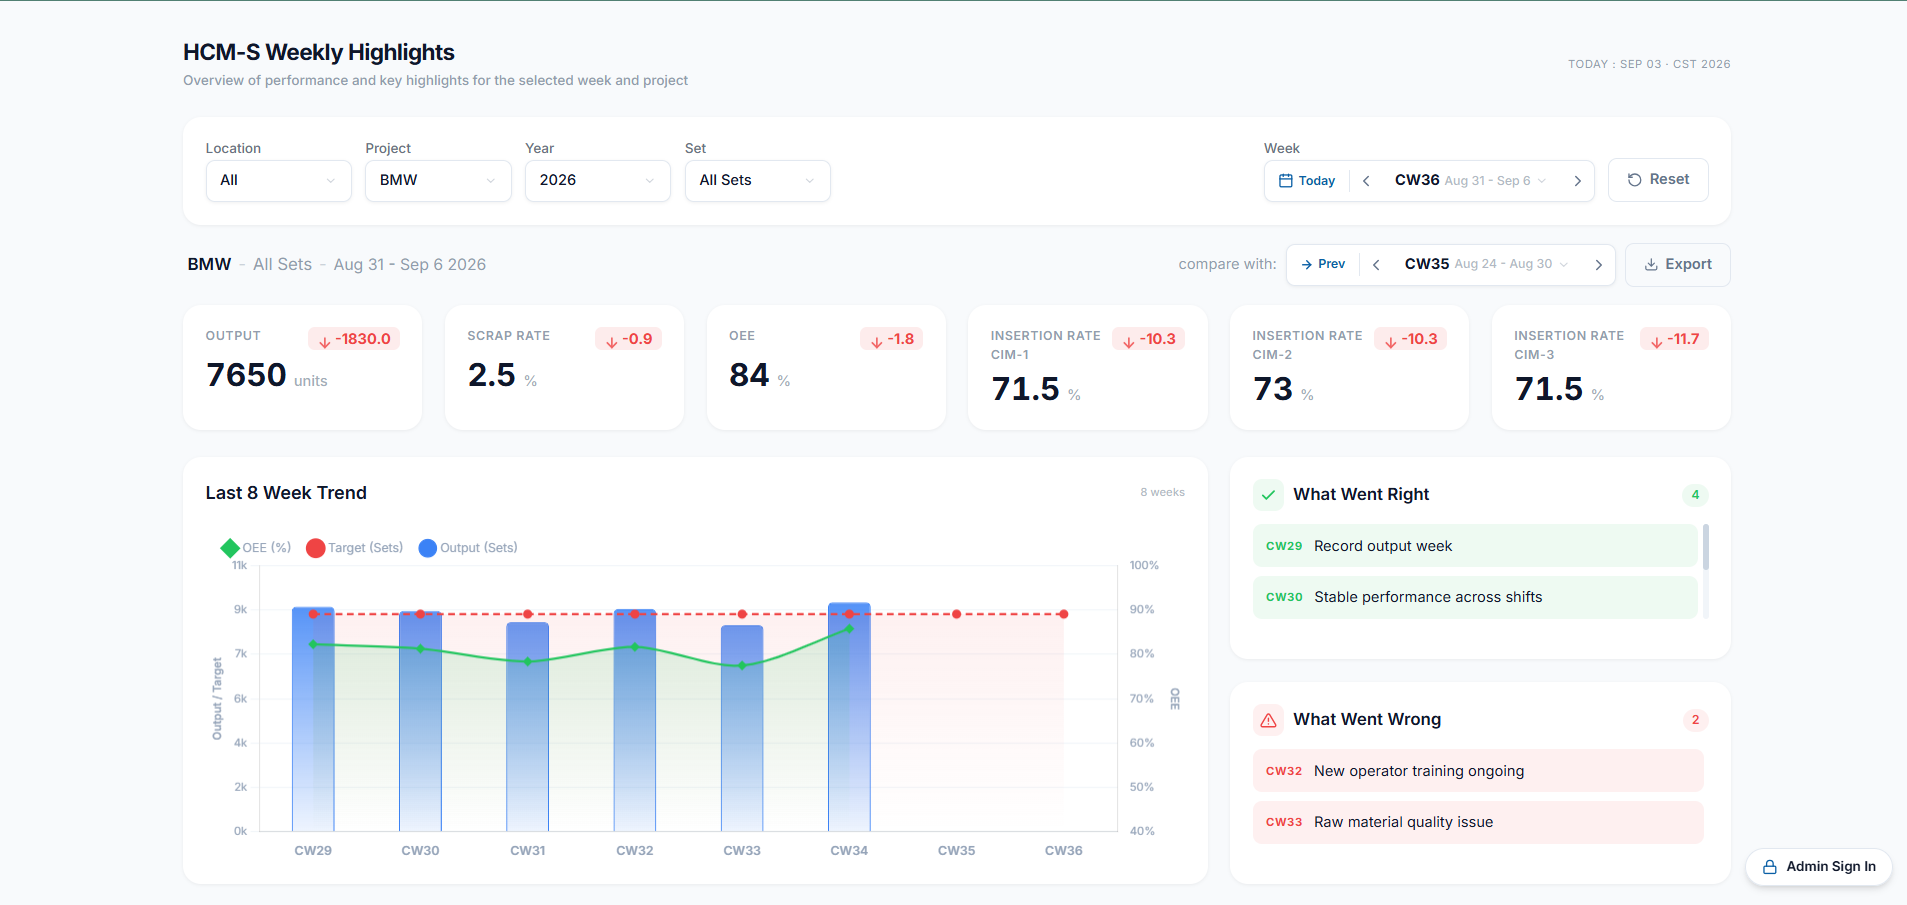
\includegraphics[width=0.9\textwidth]{images/Ch5/dashboard.png}
    \caption{Tableau de bord (Dashboard) interactif : Suivi des performances et tendances}
    \label{fig:ui_dashboard}
\end{figure}

Le tableau de bord permet de filtrer les données par Projet, Set de machines, Année et Semaine. Il affiche les deltas comparatifs et génère des graphiques d'évolution grâce au module de transformation intégré au Frontend.

\subsection{Espaces d'Administration et Saisie}

\begin{figure}[H]
    \centering
    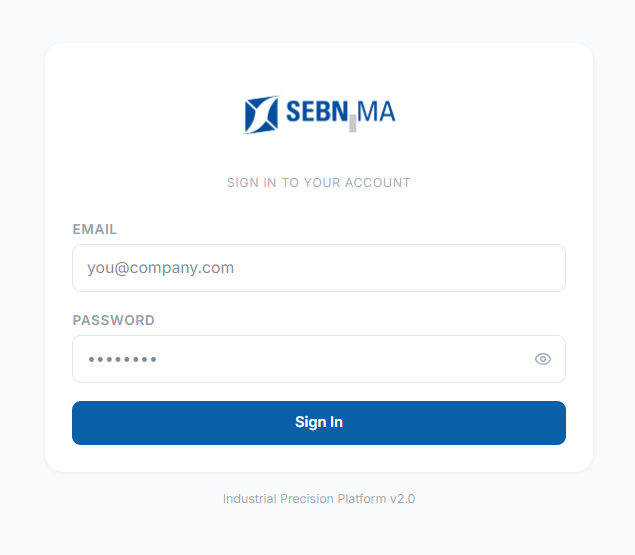
\includegraphics[width=0.6\textwidth]{images/Ch5/login.png}
    \caption{Portail d'authentification sécurisé}
    \label{fig:ui_login}
\end{figure}

\begin{figure}[H]
    \centering
    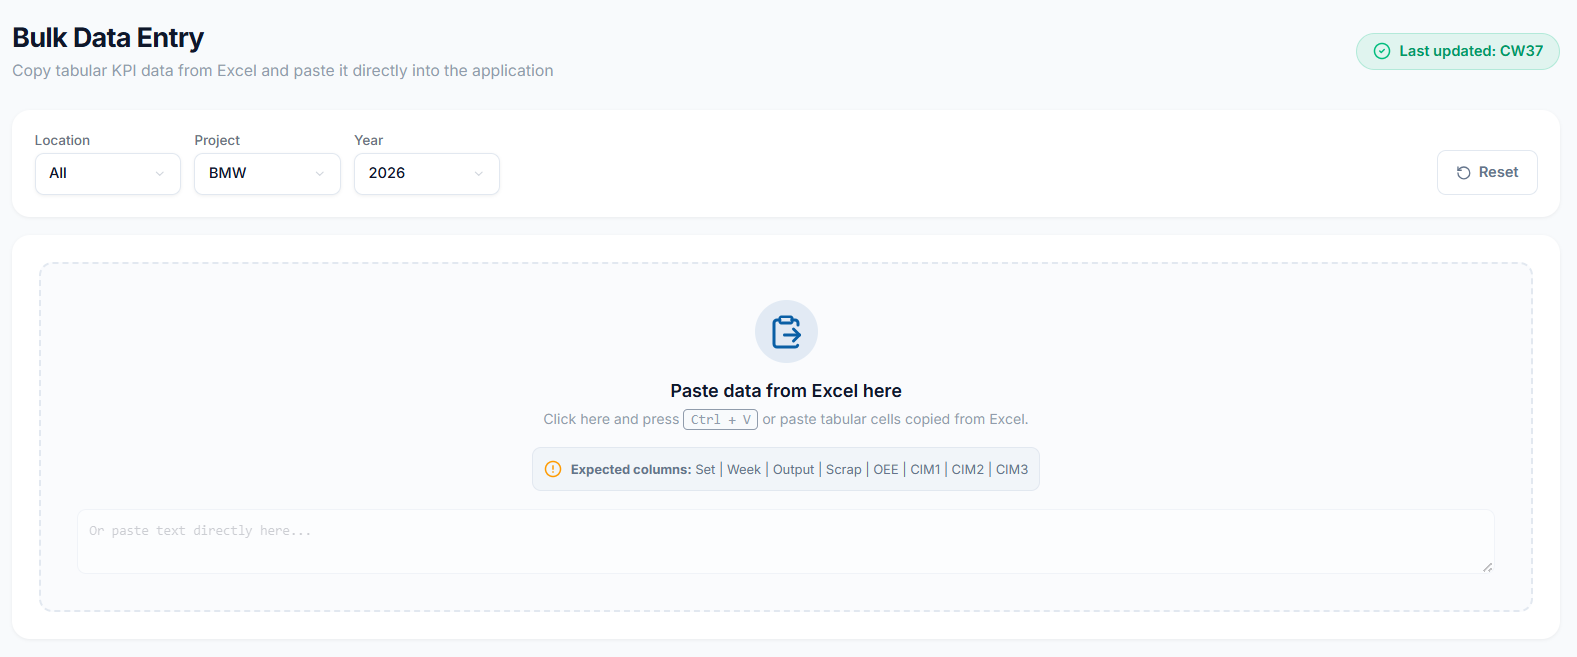
\includegraphics[width=0.9\textwidth]{images/Ch5/bulk.png}
    \caption{Interface de saisie en masse (Bulk Data Entry) avec parsing du presse-papiers Excel}
    \label{fig:ui_bulk_entry}
\end{figure}

\begin{figure}[H]
    \centering
    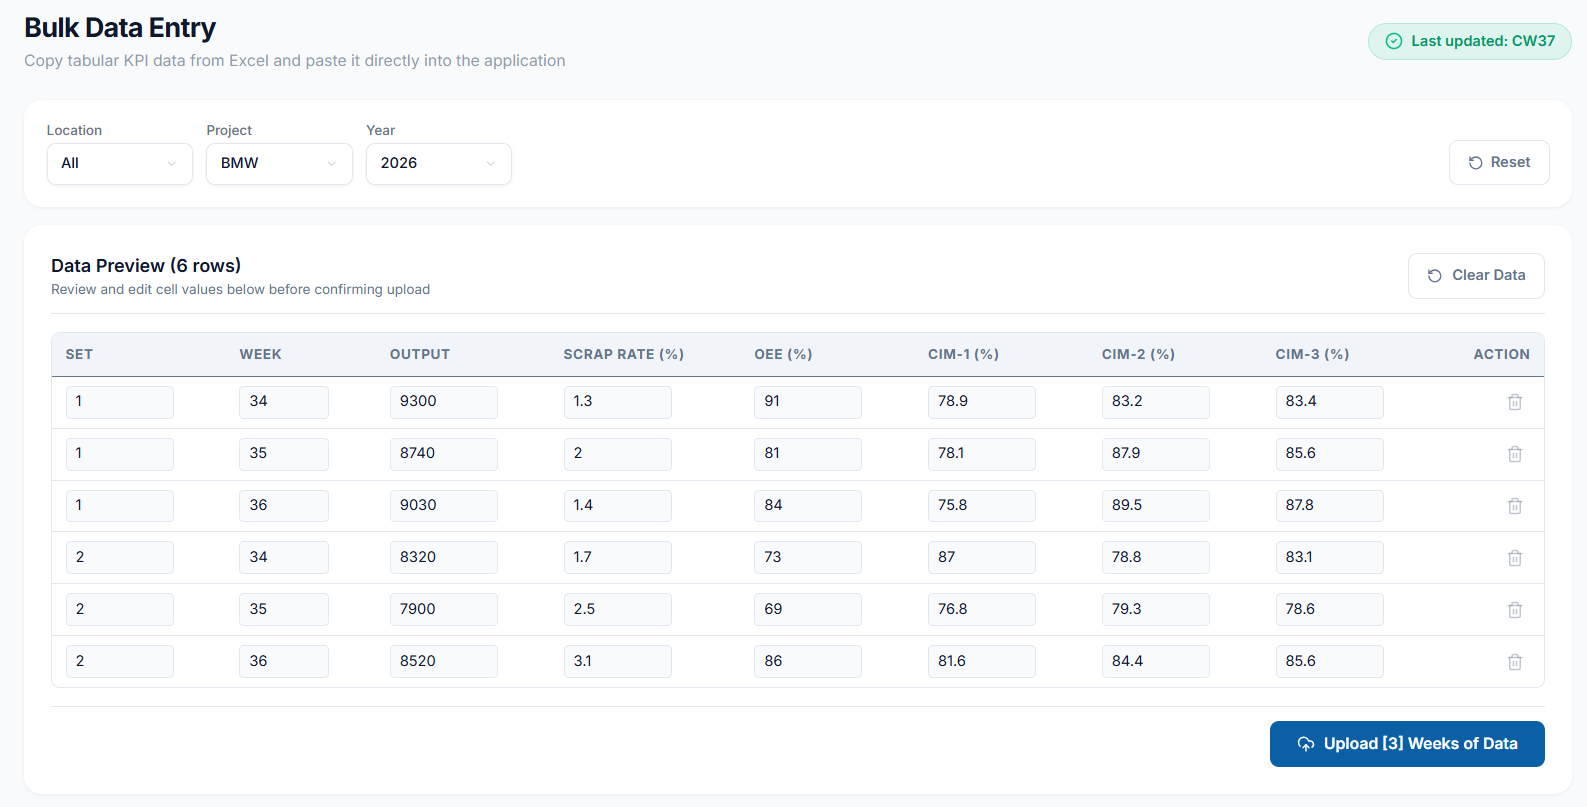
\includegraphics[width=0.9\textwidth]{images/Ch5/bulk_data.png}
    \caption{Interface de saisie en masse (Bulk Data Entry) après l'insertion des données}
    \label{fig:ui_bulk_entry_with_data}
\end{figure}

L'interface de saisie en masse a été conçue pour faciliter la transition des utilisateurs. Elle permet de copier directement les données depuis l'ancien outil Excel et de les coller dans l'application, qui valide automatiquement les formats et les numéros de semaines avant l'envoi au serveur.

\subsection{Gestion du Système (Super Admin)}

% Affichage de deux images côte à côte pour gagner de l'espace
\begin{figure}[H]
    \centering
    \begin{minipage}{0.48\textwidth}
        \centering
        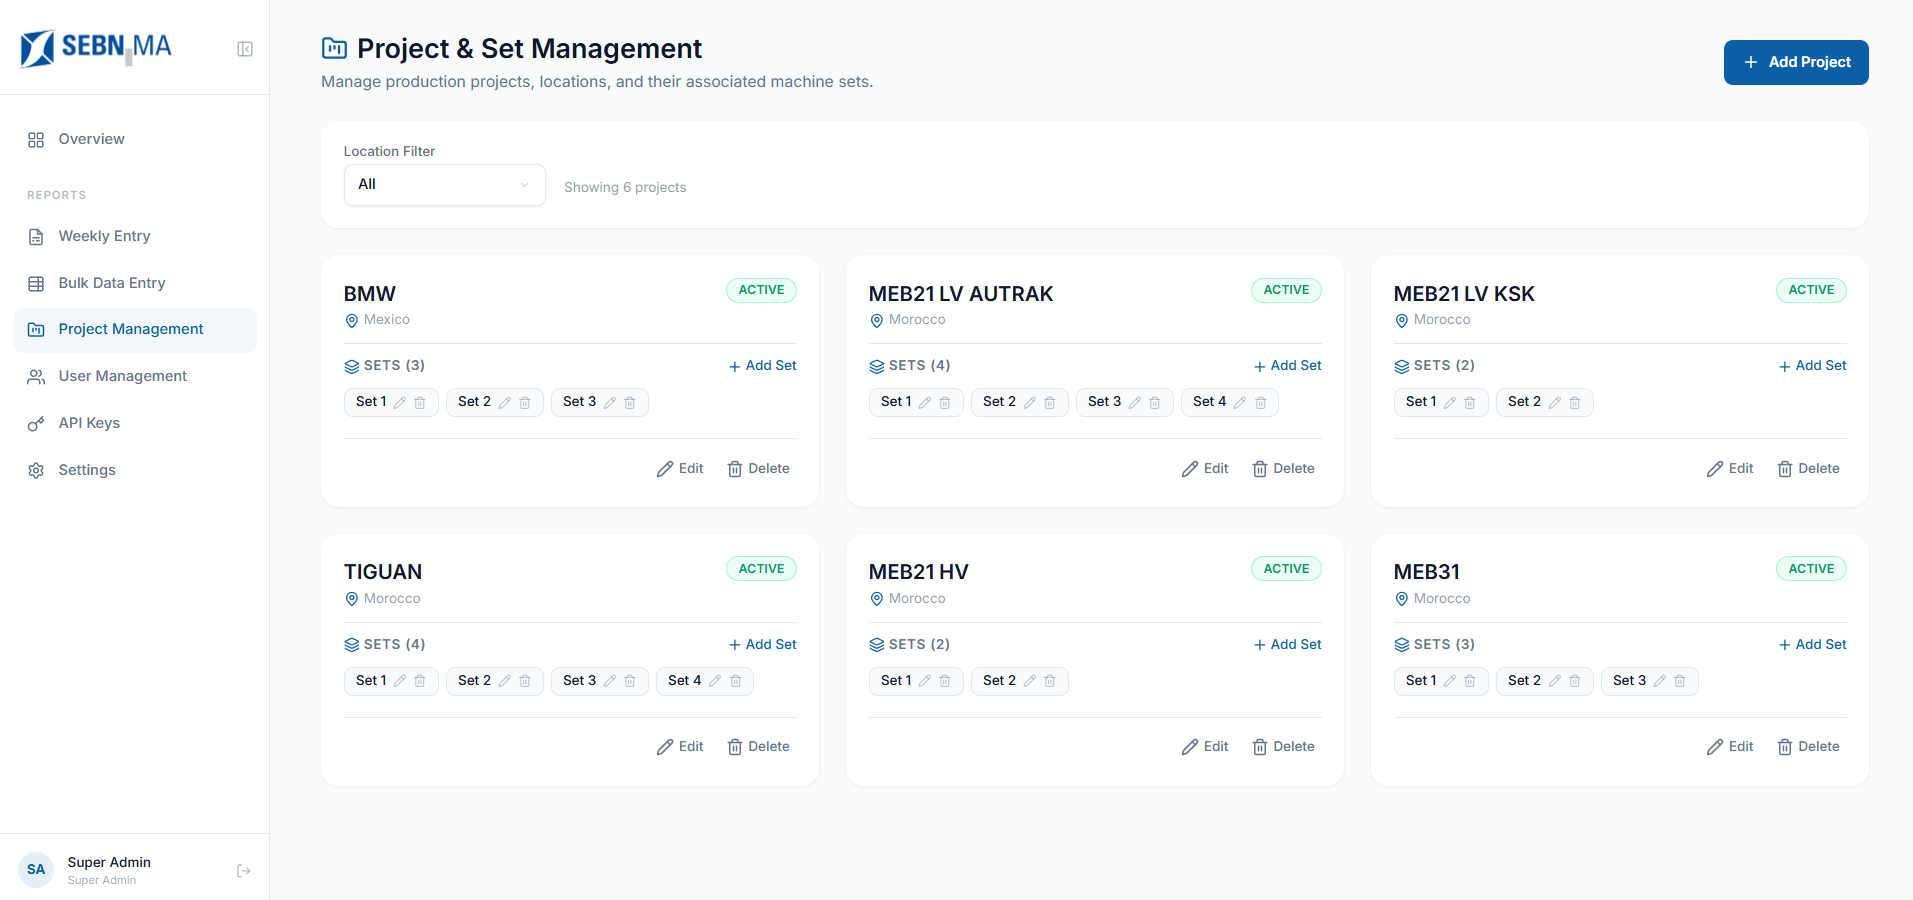
\includegraphics[width=\linewidth]{images/Ch5/projects.png}
        \caption{Gestion des Projets et des Sets machines}
        \label{fig:ui_projects}
    \end{minipage}\hfill
    \begin{minipage}{0.48\textwidth}
        \centering
        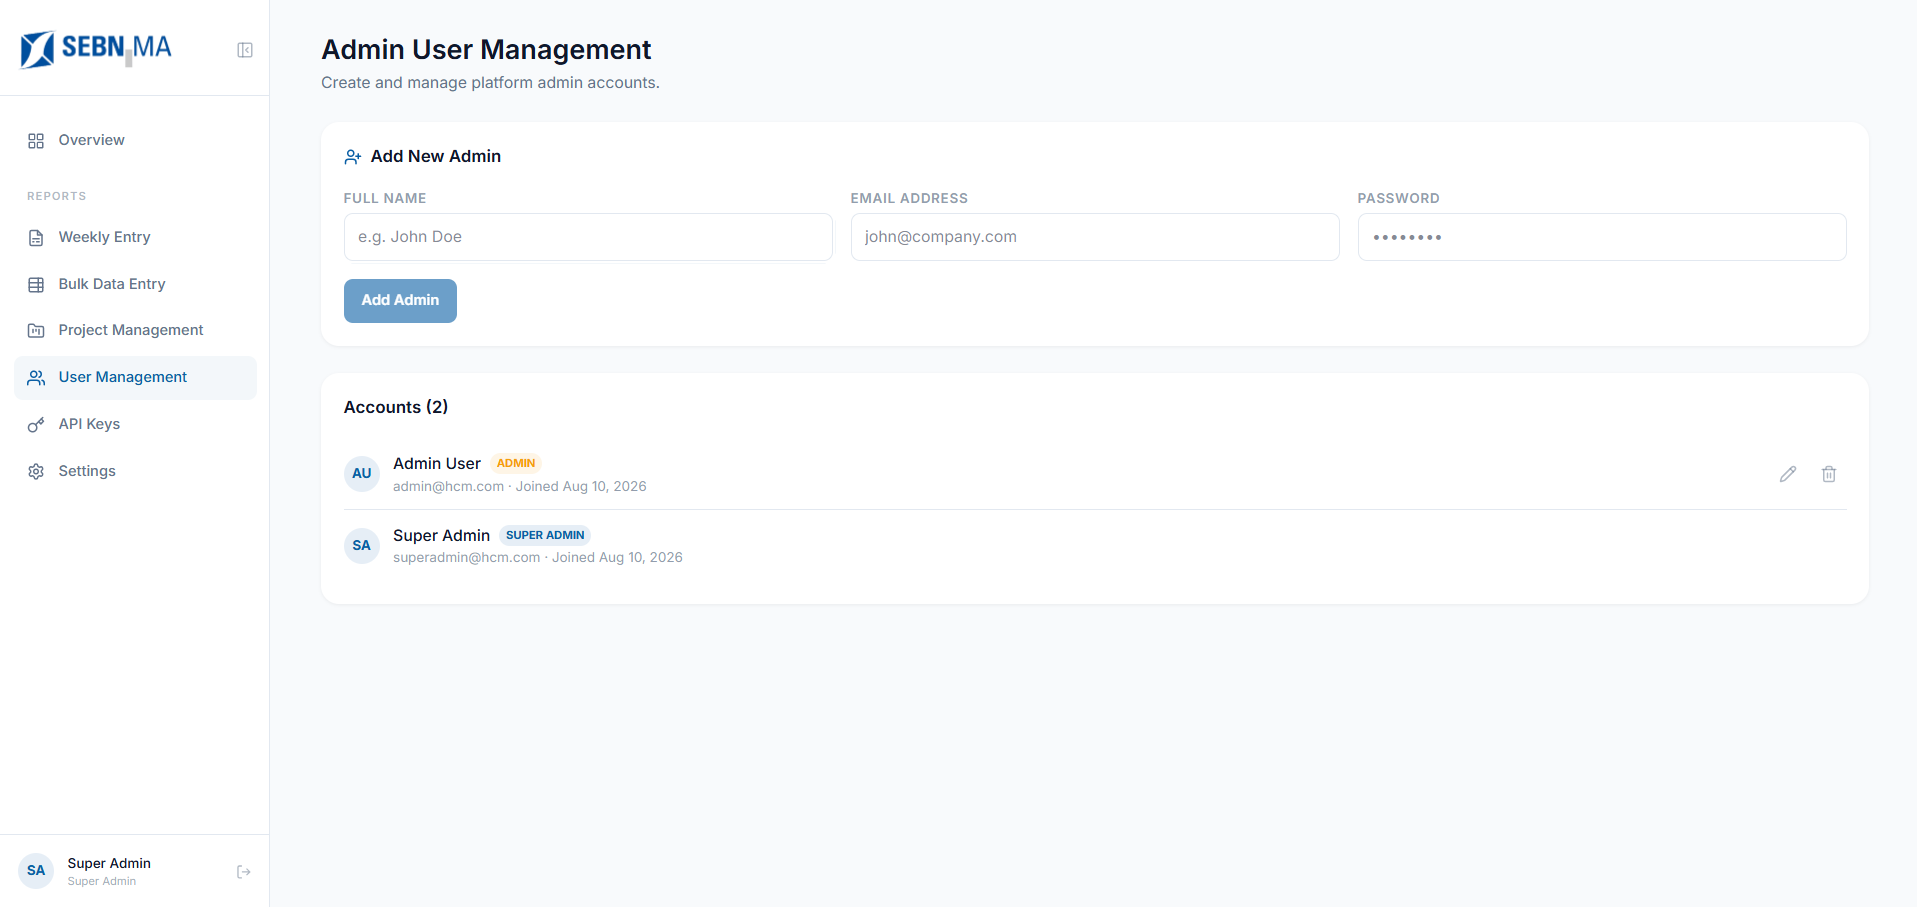
\includegraphics[width=\linewidth]{images/Ch5/users.png}
        \caption{Gestionnaire d'accès et de comptes utilisateurs}
        \label{fig:ui_admin_panel}
    \end{minipage}
\end{figure}

Les panneaux d'administration permettent la création de nouveaux projets, l'attribution des rôles utilisateurs et la génération sécurisée des clés d'API nécessaires à la macro d'automatisation (Phase 2).

% ---------------------------------------------------------
\section{Tests et Assurance Qualité}
Afin de valider la fiabilité de la solution, une stratégie de test rigoureuse a été implémentée. Le Backend est couvert par des tests automatisés via \textbf{Pytest}, s'exécutant sur une base de données SQLite en mémoire. Côté Frontend, \textbf{Vitest} vérifie la robustesse de la logique métier critique (comme le parsing du tableau Excel et le calcul des statistiques des KPIs) avant chaque déploiement.

% ---------------------------------------------------------
\section{Déploiement, Topologie d'Hébergement et Défis Réseau}
\label{sec:deploiement_infra}

\subsection{Topologie de Déploiement Actuelle (Cloud Multi-Plateforme)}
Pour des impératifs d'agilité, de rapidité d'itération et d'optimisation des coûts lors de la phase de validation, l'application a été déployée sur une infrastructure Cloud découplée et multi-fournisseurs :
\begin{itemize}
    \item \textbf{Frontend (Vercel) :} La Single Page Application React est hébergée sur la plateforme \textbf{Vercel}. Elle bénéficie d'un réseau de diffusion de contenu mondial (Edge CDN Anycast) assurant des temps de chargement minimes et un renouvellement automatique des certificats SSL/TLS.
    \item \textbf{Backend (Railway via Docker Hub) :} L'API FastAPI conteneurisée est déployée sur le PaaS \textbf{Railway}. Le service est configuré pour écouter le registre \textbf{Docker Hub}, déclenchant un redéploiement automatique dès qu'une nouvelle image est poussée par le pipeline CI/CD GitHub Actions.
    \item \textbf{Base de Données (Neon Database) :} Les données sont hébergées sur une instance PostgreSQL Serverless gérée par \textbf{Neon}. Cette solution offre une séparation du stockage et du calcul, des sauvegardes automatiques ainsi qu'un chiffrement obligatoire des connexions via SSL (\texttt{sslmode=require}).
\end{itemize}

\subsection{Contraintes du Réseau Industriel SEBN-MA}
Lors des essais d'intégration sur site, une contrainte majeure a été identifiée : la politique de sécurité informatique (IT/OT) de l'usine SEBN-MA impose un filtrage réseau strict par pare-feu (\textit{Firewall}) et proxy d'entreprise.
Les flux sortants vers des domaines publics non référencés (notamment les sous-domaines génériques de développement tels que \texttt{*.vercel.app} ou \texttt{*.railway.app}) sont automatiquement bloqués. 

Par conséquent, les ordinateurs d'atelier connectés au réseau local de l'usine ne peuvent pas communiquer directement avec les services Cloud publics. Cette restriction constitue un obstacle direct pour la \textbf{Phase 2} du projet, où les macros Excel VBA et les scripts d'automatisation situés sur les postes de travail locaux doivent transmettre les enregistrements de production à l'API.

\subsection{Solutions Stratégiques pour la Phase 2 (Mise en Production Industrielle)}
Afin de surmonter ce défi et de concrétiser l'ingestion automatisée en production, deux solutions viables ont été analysées et proposées :

\subsubsection{Solution 1 : Déploiement On-Premise avec Cloudflare Tunnel (Recommandée)}
Cette approche consiste à rapatrier l'hébergement de l'application sur un serveur physique ou une machine virtuelle interne au réseau de l'entreprise via \texttt{docker-compose} (Backend, Frontend Nginx et PostgreSQL). 

Pour rendre l'application accessible à la fois depuis le réseau local de l'usine et depuis l'extérieur (pour les managers nomades), nous préconisons l'usage d'un \textbf{Cloudflare Tunnel} (\textit{cloudflared}) :
\begin{itemize}
    \item \textbf{Sécurité à zéro port ouvert :} Le démon de tunneling établit une connexion chiffrée purement sortante (\textit{outbound}) vers les serveurs edge de Cloudflare. Aucun port entrant (\textit{inbound}) n'a besoin d'être ouvert sur le pare-feu de SEBN-MA, préservant l'étanchéité totale du réseau industriel.
    \item \textbf{Double accessibilité :} Les opérateurs sur site accèdent au tableau de bord via l'adresse IP interne (latence nulle), tandis que les utilisateurs distants y accèdent via un domaine public sécurisé protégé par le WAF (Web Application Firewall) de Cloudflare.
\end{itemize}

\subsubsection{Solution 2 : Domaine Personnalisé d'Entreprise et Whitelisting Réseau}
Si la direction informatique privilégie le maintien de l'hébergement dans le Cloud pour s'affranchir de la gestion d'un serveur local, la démarche suivante sera appliquée :
\begin{itemize}
    \item Remplacement des domaines génériques gratuits par un nom de domaine personnalisé et sécurisé propre à l'organisation (ex: \texttt{kpi-cims.sebn.com}).
    \item Soumission d'une demande de mise sur liste blanche (\textit{Whitelisting}) auprès du département réseau/sécurité de SEBN-MA afin d'autoriser les flux HTTPS vers ce domaine certifié à travers le proxy et le pare-feu de l'entreprise.
\end{itemize}

% ---------------------------------------------------------
\section*{Conclusion}
\addcontentsline{toc}{section}{Conclusion}
Cette phase de réalisation a permis de concrétiser les concepts architecturaux définis précédemment. Le choix d'outils modernes et performants (React, FastAPI, PostgreSQL), couplé à des algorithmes de sécurité avancés, a abouti à une application stable, ergonomique et hautement sécurisée. La solution déployée répond pleinement au cahier des charges de SEBN-MA, ouvrant la voie à une intégration réussie dans le cycle de production.